%!TEX root = thesis.tex
\chapter{Motivation and Backgroud}

\section{\aclp{PAC}}
\aclp{PAC} are a relatively new class of controllers emerged in the past years
out of the discussion on advantages and disadvantages of \acp{PLC} compared to
\acp{PC} \citep{bel05}. The acronym \ac{PAC} itself was introduced by the
\ac{ARC} in 2001 \citep{pay13} to represent this next generation controllers.
However, a strict definition to clearly identify a \ac{PAC} and differentiate
it from other \acp{PLC} is missing. The term is used more as buzzword for the
automation vendor's marketing, but still reflects the increasing demands by
the modern industry and the evolution of automation controllers. 

Since its origin in the 1960s \citep{par99}, the \ac{PLC} dominates the
control and automation market by providing high reliability, a well-known
programming model and industrial I/O. It is used for various automation tasks
in typically electromechanical processes, for example machinery or plant
control. Inspired by the hand-wired relay logic systems and wire-diagrams, the
ladder-logic programming eased the transition to the new technology. Figure
\ref{fig:plc} shows the basic structure of a \ac{PLC} consisting out of input
and output ports and a program, implementing the control logic.
\begin{figure}
	\centering
	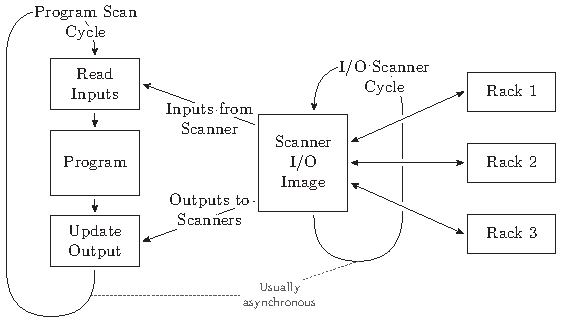
\includegraphics[width=6cm]{../figures/plc}
	\caption{The \acs{PLC} program scan \citep[adapted from][]{par99}}
	\label{fig:plc}
\end{figure}
The input ports are typically connected to different sensors, for example
light barriers, level indicators or temperature sensors, while the output
ports control actuators like contactors or valves. Each time the program scan
is executed, the inputs are read and fed into the control logic, updating the
output ports accordingly. Note, that a \ac{PLC} does not control the system
continuously, but typically at a frequency of several $\SI{}{\kilo\hertz}$
\citep{par99}.

While the \ac{PLC} structure was designed for basic machine control, it
reaches its limits for more advanced applications requiring, for example,
extensive analog I/O, network connectivity, or enterprise integration. Back in
the 1980s and 1990s around 80\% of the industry's applications were solved by
traditional \acp{PLC} \citep{bel05}. This resulted in a growth of low-cost
systems and a discontinuity in controller technology. Engineers, targeting the
20\% of feature-rich applications, pushed the classical designs to its limits
and started evaluating different technology. They came up with \acp{PC} for
industrial control, offering advanced software capabilities, utilization of
\ac{COTS} components and graphical environments \citep{bel05}. However,
standard \acp{PC} are not ideal for industrial control applications due to
missing robustness in rugged environments, stable operating systems and common
programming. Finally, the engineers either omitted advanced functionalities or
deployed a coupled \ac{PC}/\ac{PLC} system. Without any satisfactory solution,
hardware vendors tried to fill up the gap by developing a new class of
controller, the so-called \acp{PAC}.

The \ac{PAC} combines the best features of \acp{PLC} and \acp{PC} in a single
device by incorporating robustness and reliability with advanced software
capabilities as illustrated in figure \ref{fig:pac}.
\begin{figure}
	\centering
	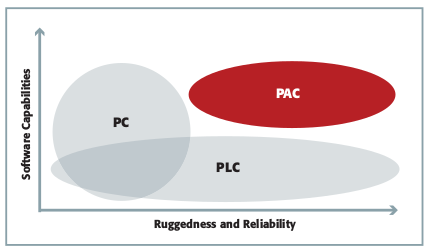
\includegraphics[width=6cm]{../figures/pac}
	\caption{\acsp{PAC} compared to \acsp{PLC} and \acsp{PC} \citep[adapted from][]{bel05}}
	\label{fig:pac}
\end{figure}
However, vendors pursue different strategies to provide the advanced software
for complex applications. \citep{bel05}. Traditional \ac{PLC} companies
adjusted the existing scanning architecture and extended it by new
functionality. While the well-known architecture provides short development
cycles and eliminates the need of low-level knowledge by the engineers, it
still limits the flexibility and customizability of the system. On the other
hand, \ac{PC} vendors addressed the demand for advanced features by starting
with a general-purpose programming environment, which provides access to the
internals of the system and abstractions for commonly used operations. While
this approach allows extremely flexible solutions, it lacks the familiar
\ac{PLC} programming architecture, making application development more
demanding.

The flexible software architecture introduced for the \acp{PAC} enables
engineers to implement complex applications, without being restricted to a
fixed device structure. However, software implementations reach their limits
for high-performance or low-latency applications. These demands typically
result in custom hardware design utilizing direct I/O connections and parallel
processing. While \acp{ASIC} are often not financially viable, \acp{FPGA} are
getting more and more ubiquitous \citep{VMB13}. \acp{FPGA} consist out of
configurable logic, interconnect and I/O blocks, which can be programmed to
implement arbitrary logic. While this technology seems to perfectly fit into
the concept of \acp{PAC}, especially with upcoming integrated \acp{SoC}, it is
limited to hardware designers capable of programming in low-level languages
like \ac{VHDL} and understanding the architecture of the underlying system.
Efficiently programming such a hybrid system requires a high-level abstraction
of hardware and software resources \citep{ANA04} and a unified programming
environment. Both topics are part of ongoing research including programming
models for hybrid multi-core systems and high-level specifications of hardware
logic.

\section{ReconOS for Hybrid Multi-Core Systems}
With increasing demand for high-performance embedded systems and upcoming
\acp{SoC} integrating powerful general-purpose processors with reconfigurable
logic, convenient programming models are required to tap the full potential of
these hybrid systems \citep{ANA04,VMB13}. \ac{HLS} approaches allow the
synthesis of hardware designs from a high-level language and simplify the
development of custom hardware, but do not provide an abstraction for the
underlying hardware components at system level. 

ReconOS addresses this problem and provides a unified execution environment
leveraging the well-established multithreaded programming model and extends an
\ac{OS} with hardware thread support \citep{AHK14}. The multithreaded
programming model is highly accepted in the software engineering community and
suitable for embedded applications \citep{ANA04} composed of concurrently
running threads, synchronizing and exchanging data via standardized \ac{OS}
mechanism, for example semaphores, mutexes or message queues. The threads
specified by the system developer are transparent against their implementation
and distributed across the \ac{CPU} and \ac{FPGA} resources, while having
symmetrical access to all communication mechanisms. Figure
\ref{fig:reconos_model} illustrated the concept of hardware and software
threads communicating via a standardized \ac{OS} interface.
\begin{figure}
	\centering
	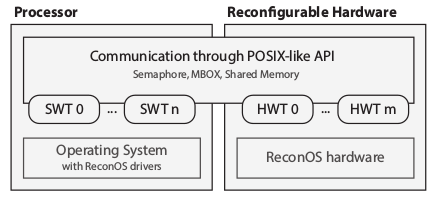
\includegraphics[width=6cm]{../figures/reconos_model}
	\caption{The ReconOS programming model}
	\label{fig:reconos_model}
\end{figure}
This approach reduces development costs since the application structure
remains at a high level and the partitioning can be changed during development
without additional effort. Furthermore, the applications are portable between
different platforms, due to the defined \ac{OS} interface \citep{AHK14}.

To illustrate the concept of a ReconOS thread, consider the exemplary thread
in listing \ref{lst:swt}. It receives data via an incoming mailbox, processes
this data internally and writes back the result to an outgoing mailbox.
\begin{lstlisting}[
	language=C,
	caption={Exemplary ReconOS thread in C},
	label={lst:swt},
	morekeywords={THREAD_ENTRY}
]
#include "reconos_thread.h"
#include "reconos_calls.h"

THREAD_ENTRY() {
	data_t data;

	while(1) {
		data = mbox_get(resources_mbox_in);
		process(data);
		mbox_put(resources_mbox_out, data);
	}
}
\end{lstlisting}

%To support a transparent multithreading across the hardware/software boundary,
%ReconOS implements a runtime as shown in figure \ref{fig:reconos_runtime}.
%\begin{figure}
%	\centering
%	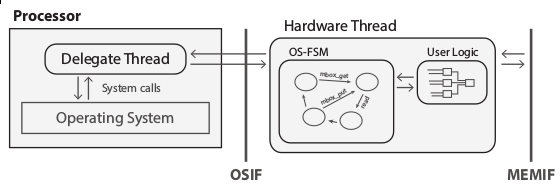
\includegraphics[width=6cm]{../figures/reconos_hwt}
%	\caption{The ReconOS runtime}
%	\label{fig:reconos_runtime}
%\end{figure}

\section{High Level Synthesis}

\section{Contribution of this Work}
Due to the promising perspective for the use of reconfigurable device  in
\acp{PAC} and the ongoing research in hybrid multi-core systems, this thesis
tries to evaluate the feasibility of such an approach. Within the scope of its
research on multi-core systems, the University of Paderborn is developing a
multithreaded framework called ReconOS, abstracting the hardware/software
boundary and providing a convenient programming model. 